\begin{apendicesenv}

\chapter{Prompts utilizados no experimento}
\label{ap:prompts-execucao}

Este apêndice reúne exemplos representativos das quatro configurações de prompt empregadas na etapa de execução do experimento. A tabela a seguir resume a organização desses prompts por tipo de trecho e versão. A versão completa dos prompts está disponível no arquivo \textit{Script-Api-LLMs/prompts.json} do repositório de execução do trabalho no GitHub\footref{fn:repo}.

\begin{longtable}{p{0.18\textwidth} p{0.18\textwidth} p{0.18\textwidth} p{0.36\textwidth}}
\caption{Resumo dos prompts utilizados no experimento}\label{tab:resumo-prompts}\\
\hline
Tipo & Versão & Smells avaliados & Identificação do exemplo \\
\hline
\endfirsthead
\hline
Tipo & Versão & Smells avaliados & Identificação do exemplo \\
\hline
\endhead
Classe & Zero-shot & Blob/God Class e Data Class & Exemplo com o sample 3698323, sem definições adicionais \\
Classe & Few-shot & Blob/God Class e Data Class & Exemplo com o sample 3698323, com definições e exemplos conceituais \\
Método & Zero-shot & Long Method e Feature Envy & Exemplo com o sample 6863460, sem definições adicionais \\
Método & Few-shot & Long Method e Feature Envy & Exemplo com o sample 6863460, com definições e exemplos conceituais \\
\hline
\end{longtable}

\section{Prompt zero-shot para classe}

\begin{verbatim}
Você é especialista em qualidade de código Java.

Analise a classe abaixo e responda:

Blob: SIM ou NÃO
Data Class: SIM ou NÃO

Código:
public interface PlaybackNearlyFinishedRequestHandler extends RequestHandler {

	boolean canHandle(HandlerInput input, PlaybackNearlyFinishedRequest playbackNearlyFinishedRequest);

	Optional<Response> handle(HandlerInput input, PlaybackNearlyFinishedRequest playbackNearlyFinishedRequest);

	@Override
	default boolean canHandle(HandlerInput handlerInput) {
		if (handlerInput.getRequest() instanceof PlaybackNearlyFinishedRequest) {
			return canHandle(handlerInput, (PlaybackNearlyFinishedRequest)handlerInput.getRequest());
		}
		return false;
	}

	@Override
	default Optional<Response> handle(HandlerInput handlerInput) {
		return handle(handlerInput, (PlaybackNearlyFinishedRequest)handlerInput.getRequest());
	}
}
\end{verbatim}

\section{Prompt few-shot para classe}

\begin{verbatim}
Você é especialista em qualidade de código Java.

Definições:
- Blob: classe com responsabilidades excessivas, concentrando muitas funções ou coordenando múltiplos aspectos do sistema.
- Data Class: classe focada principalmente em armazenar dados, com pouca ou nenhuma lógica de negócio relevante.

Exemplo 1:
Código:
public class OrderManager {
	private List<Order> orders;
	private DatabaseConnection dbConnection;
	private EmailService emailService;
	private PaymentGateway paymentGateway;
	private TaxCalculator taxCalculator;
	private ReportingService reportingService;

	public void createOrder(Order order) { /* implementação complexa */ }
	public void validateUser(String userId) { /* implementação complexa */ }
	public void processPayment(PaymentInfo payment) { /* implementação complexa */ }
	public void sendConfirmationEmail(String email) { /* implementação complexa */ }
	public void generateMonthlySalesReport() { /* implementação complexa */ }
	public double calculateTotalTax(double subtotal) { /* implementação complexa */ }
}

Resposta:
Blob: SIM
Data Class: NÃO

Exemplo 2:
Código:
public class Point {
	public double x;
	public double y;

	public Point(double x, double y) {
		this.x = x;
		this.y = y;
	}
}

Resposta:
Blob: NÃO
Data Class: SIM

Agora analise a classe abaixo.

Responda apenas com:
Blob: SIM ou NÃO
Data Class: SIM ou NÃO
Sem explicações adicionais.

Código:
public interface PlaybackNearlyFinishedRequestHandler extends RequestHandler {

	boolean canHandle(HandlerInput input, PlaybackNearlyFinishedRequest playbackNearlyFinishedRequest);

	Optional<Response> handle(HandlerInput input, PlaybackNearlyFinishedRequest playbackNearlyFinishedRequest);

	@Override
	default boolean canHandle(HandlerInput handlerInput) {
		if (handlerInput.getRequest() instanceof PlaybackNearlyFinishedRequest) {
			return canHandle(handlerInput, (PlaybackNearlyFinishedRequest)handlerInput.getRequest());
		}
		return false;
	}

	@Override
	default Optional<Response> handle(HandlerInput handlerInput) {
		return handle(handlerInput, (PlaybackNearlyFinishedRequest)handlerInput.getRequest());
	}
}
\end{verbatim}

\section{Prompt zero-shot para método}

\begin{verbatim}
Você é especialista em qualidade de código Java.

Analise o método abaixo:

Long Method: SIM ou NÃO
Feature Envy: SIM ou NÃO

Código:
private void colorLoops() {
  try {
	for (final INaviViewNode currentNode : getGraph().getNodes()) {
	  if (currentNode.getParents().isEmpty()) {
		CLoopHighlighter.colorLoops(getGraph(), currentNode);
		break;
	  }
	}
  } catch (final MalformedGraphException exception) {
	NaviLogger.warning("Error: Graph is malformed, can not color loops");
  }
}
\end{verbatim}

\section{Prompt few-shot para método}

\begin{verbatim}
Você é especialista em qualidade de código Java.

Definições:
- Long Method: método muito longo, denso ou com muitas etapas, decisões e responsabilidades concentradas.
- Feature Envy: método que depende mais de dados ou comportamentos de outra classe ou objeto do que da própria classe.

Exemplo 1:
Código:
public String statement() {
	double totalAmount = 0;
	int frequentRenterPoints = 0;
	Enumeration rentals = _rentals.elements();
	String result = "Rental Record for " + name() + "\n";

	while (rentals.hasMoreElements()) {
		double thisAmount = 0;
		Rental each = (Rental) rentals.nextElement();

		switch (each.getMovie().getPriceCode()) {
			case Movie.REGULAR:
				thisAmount += 2;
				if (each.getDaysRented() > 2)
					thisAmount += (each.getDaysRented() - 2) * 1.5;
				break;
			case Movie.NEW_RELEASE:
				thisAmount += each.getDaysRented() * 3;
				break;
		}

		frequentRenterPoints++;
		if ((each.getMovie().getPriceCode() == Movie.NEW_RELEASE) && each.getDaysRented() > 1)
			frequentRenterPoints++;

		result += "\t" + each.getMovie().getTitle() + "\t" + String.valueOf(thisAmount) + "\n";
		totalAmount += thisAmount;
	}
	return result;
}

Resposta:
Long Method: SIM
Feature Envy: NÃO

Exemplo 2:
Código:
public class GradeAnalyzer {
	private Student student;

	public double calculateFinalGrade() {
		List<Grade> grades = student.getGrades();
		if (grades.isEmpty()) return 0;

		double totalEarned = 0;
		double totalPossible = 0;

		for (Grade grade : grades) {
			if (grade.isLateSubmission()) {
				totalEarned += grade.getScore() * 0.9;
			} else {
				totalEarned += grade.getScore();
			}
			totalPossible += grade.getTotalPoints();
		}
		return (totalEarned / totalPossible) * 100;
	}
}

Resposta:
Long Method: NÃO
Feature Envy: SIM

Agora analise o método abaixo.

Responda apenas com:
Long Method: SIM ou NÃO
Feature Envy: SIM ou NÃO
Sem explicações adicionais.

Código:
private void colorLoops() {
  try {
	for (final INaviViewNode currentNode : getGraph().getNodes()) {
	  if (currentNode.getParents().isEmpty()) {
		CLoopHighlighter.colorLoops(getGraph(), currentNode);
		break;
	  }
	}
  } catch (final MalformedGraphException exception) {
	NaviLogger.warning("Error: Graph is malformed, can not color loops");
  }
}
\end{verbatim}

\chapter{Evidências visuais do SonarQube}
\label{ap:sonar-evidencias}

Este apêndice reúne capturas de tela que documentam a configuração do projeto no SonarQube e a ativação das quatro regras customizadas empregadas no experimento.

\begin{figure}[H]
\centering
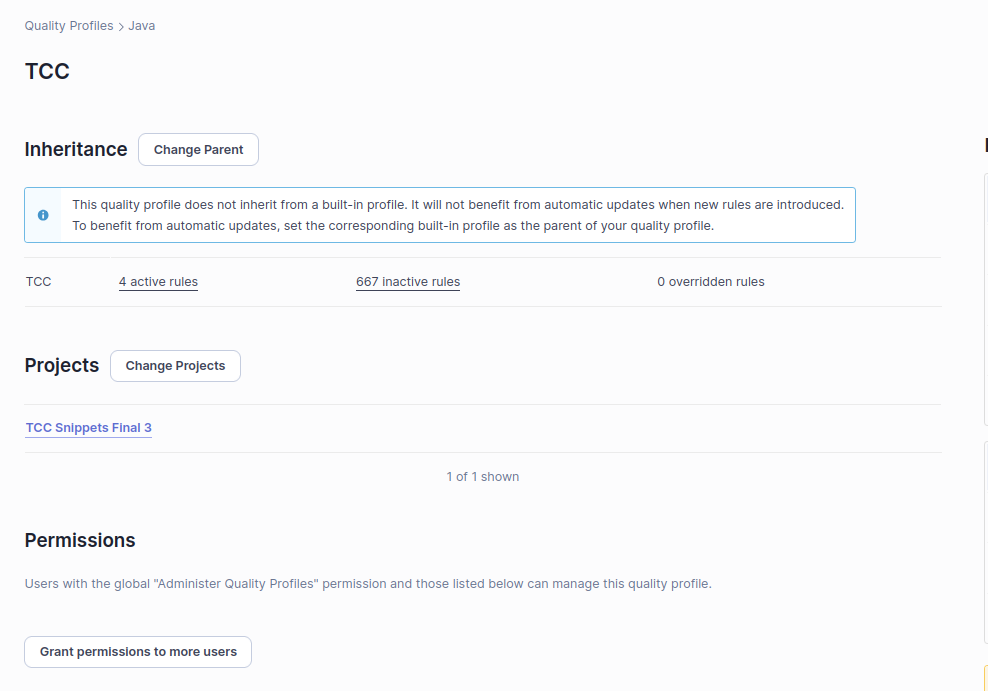
\includegraphics[width=1\textwidth]{figuras/projetosonar.png}
\caption{Projeto configurado no SonarQube com as regras customizadas ativas}
\label{fig:sonar-projeto}
\end{figure}

\begin{figure}[H]
\centering
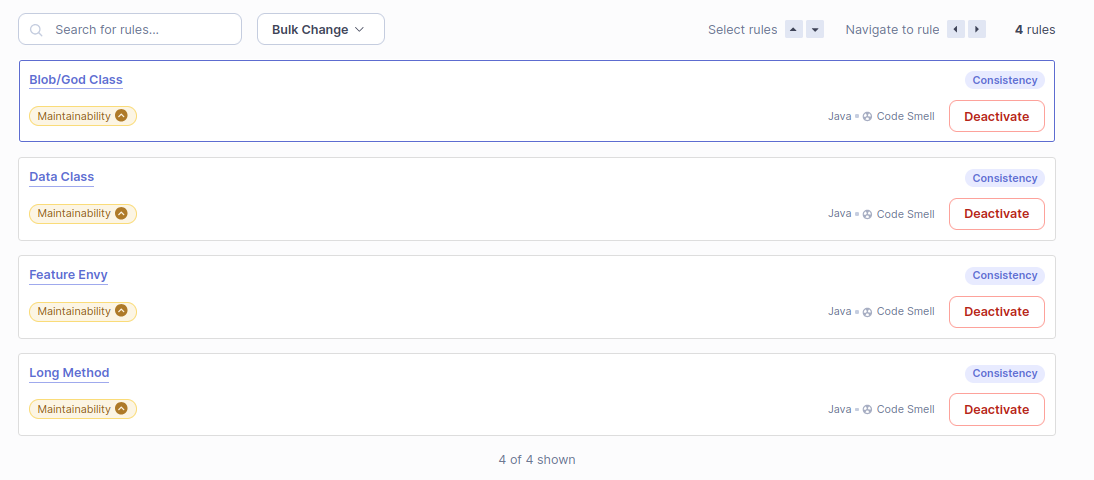
\includegraphics[width=1\textwidth]{figuras/pluginssonar.png}
\caption{Regras customizadas ativas}
\label{fig:sonar-plugins}
\end{figure}

\begin{figure}[H]
\centering
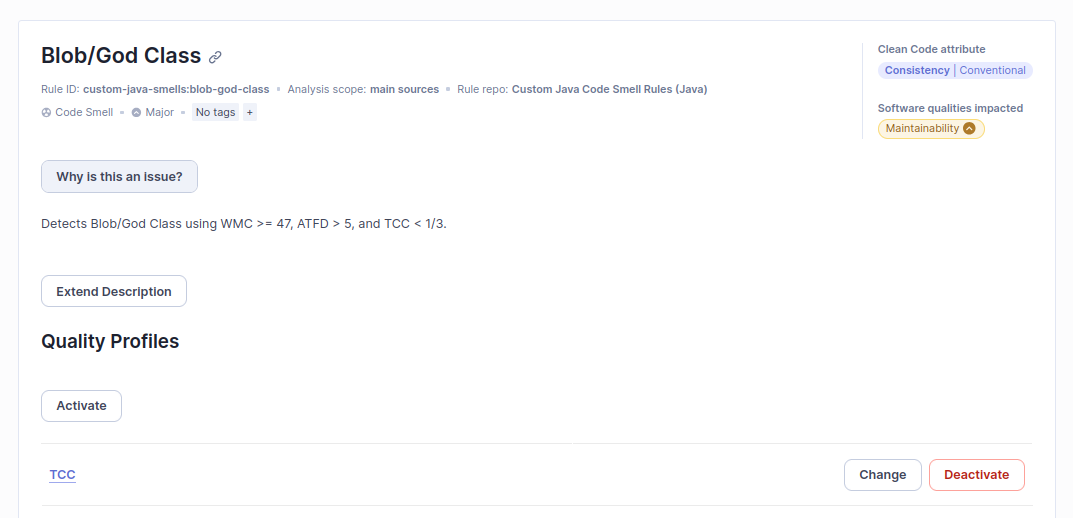
\includegraphics[width=1\textwidth]{figuras/blobsonar.png}
\caption{Regra customizada para Blob/God Class no SonarQube}
\label{fig:sonar-blob}
\end{figure}

\begin{figure}[H]
\centering
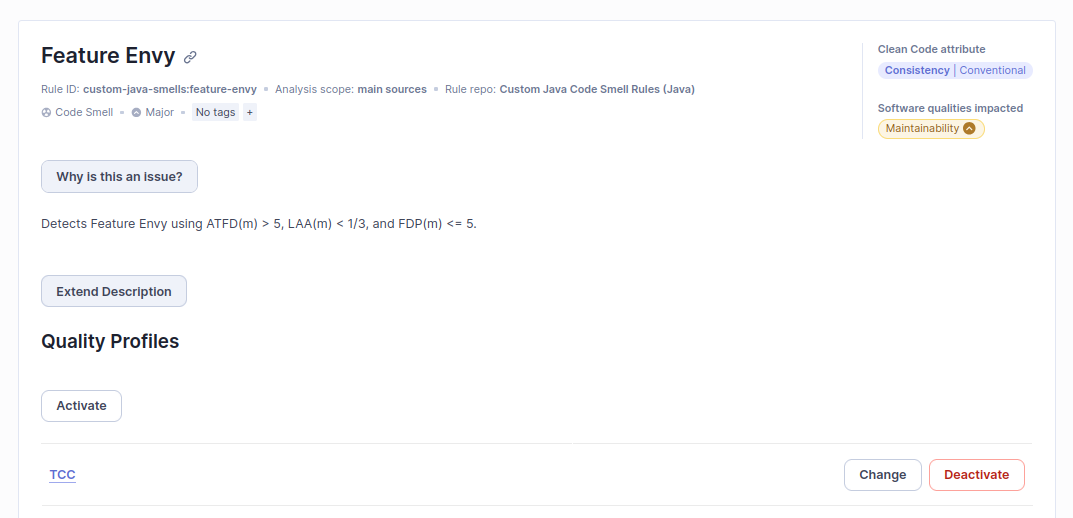
\includegraphics[width=1\textwidth]{figuras/envysonar.png}
\caption{Regra customizada para Feature Envy no SonarQube}
\label{fig:sonar-envy}
\end{figure}

\begin{figure}[H]
\centering
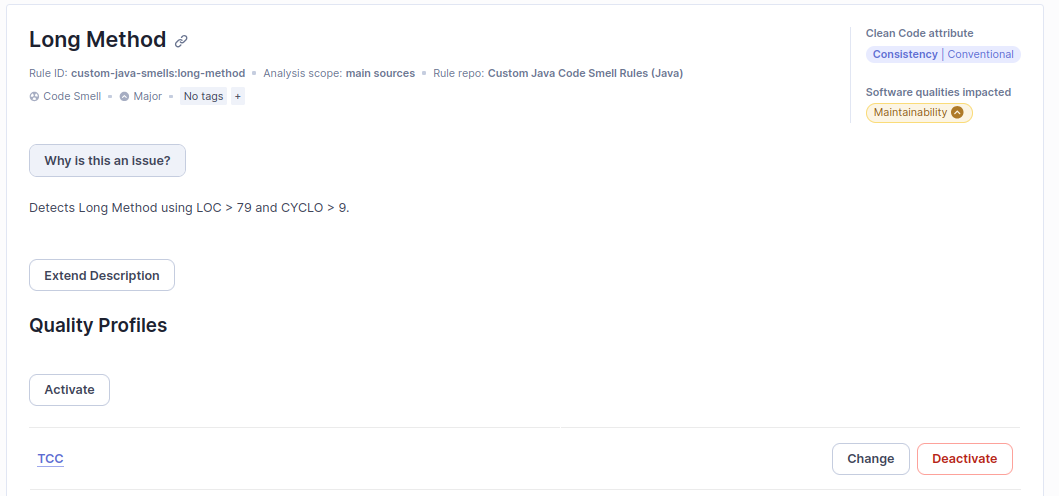
\includegraphics[width=1\textwidth]{figuras/longsonar.png}
\caption{Regra customizada para Long Method no SonarQube}
\label{fig:sonar-long}
\end{figure}

\begin{figure}[H]
\centering
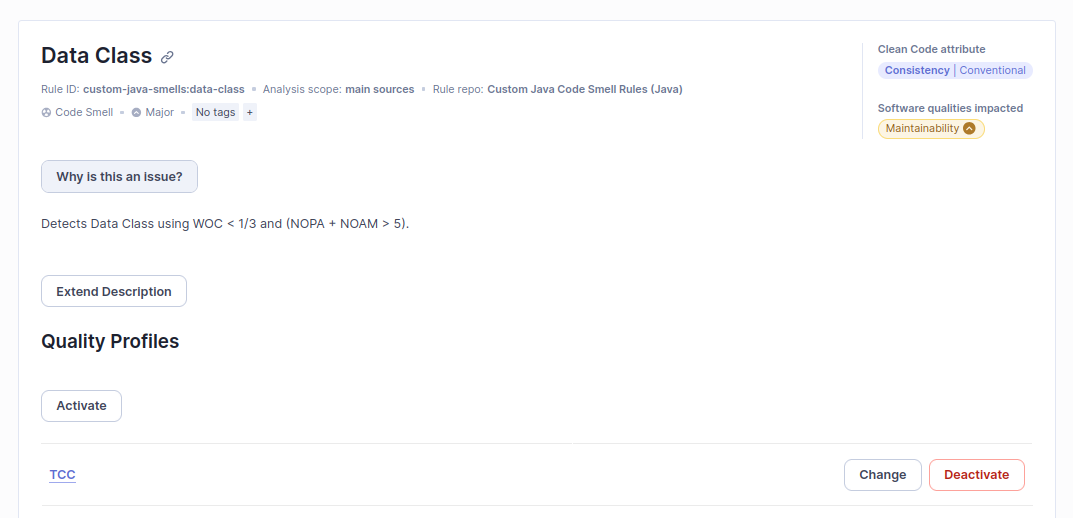
\includegraphics[width=1\textwidth]{figuras/dataclasssonar.png}
\caption{Regra customizada para Data Class no SonarQube}
\label{fig:sonar-dataclass}
\end{figure}

\end{apendicesenv}